\section{概要}
本実験の全体の流れを説明する.実験の概要を図\ref{fig:ml-flow}に示す.

\begin{enumerate}
  \item 実験に用いるデータセットを選定する.
  \item データセットを用いて,既存手法と提案手法の分類精度を比較する.
  \item 提案手法のパラメータを変更することで,分類精度にどのような影響があるかを調査する.
\end{enumerate}

\begin{figure}[htbp]  
  \centering
  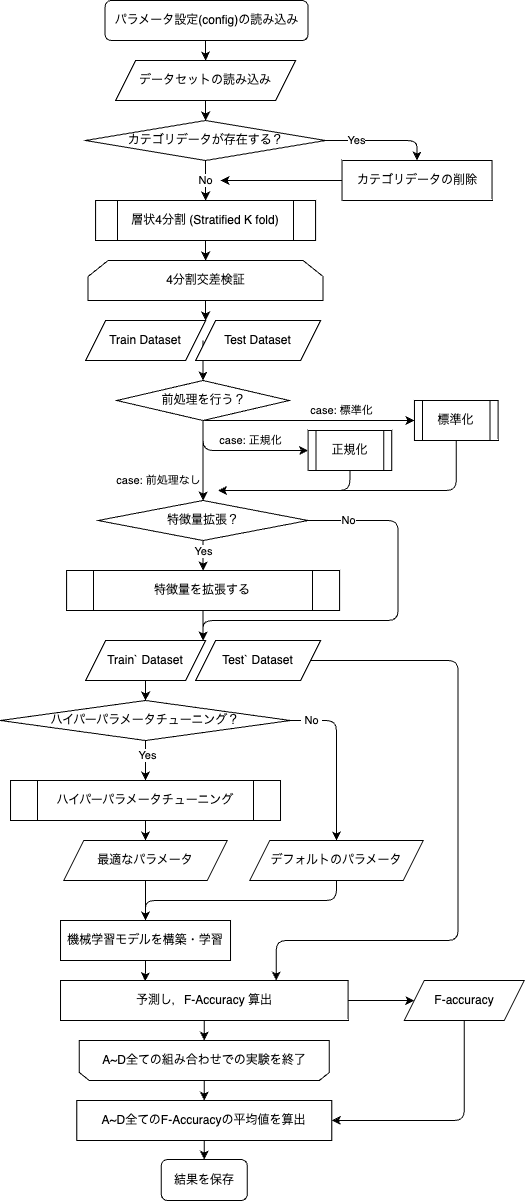
\includegraphics[width=0.6\linewidth\centering]{figures/ml-flow.png}
  \caption{実験の機械学習フロー}
  \label{fig:ml-flow}
\end{figure}
